
%% bare_conf_compsoc.tex
%% V1.4b
%% 2015/08/26
%% by Michael Shell
%% See:
%% http://www.michaelshell.org/
%% for current contact information.
%%
%% This is a skeleton file demonstrating the use of IEEEtran.cls
%% (requires IEEEtran.cls version 1.8b or later) with an IEEE Computer
%% Society conference paper.
%%
%% Support sites:
%% http://www.michaelshell.org/tex/ieeetran/
%% http://www.ctan.org/pkg/ieeetran
%% and
%% http://www.ieee.org/

%%*************************************************************************
%% Legal Notice:
%% This code is offered as-is without any warranty either expressed or
%% implied; without even the implied warranty of MERCHANTABILITY or
%% FITNESS FOR A PARTICULAR PURPOSE! 
%% User assumes all risk.
%% In no event shall the IEEE or any contributor to this code be liable for
%% any damages or losses, including, but not limited to, incidental,
%% consequential, or any other damages, resulting from the use or misuse
%% of any information contained here.
%%
%% All comments are the opinions of their respective authors and are not
%% necessarily endorsed by the IEEE.
%%
%% This work is distributed under the LaTeX Project Public License (LPPL)
%% ( http://www.latex-project.org/ ) version 1.3, and may be freely used,
%% distributed and modified. A copy of the LPPL, version 1.3, is included
%% in the base LaTeX documentation of all distributions of LaTeX released
%% 2003/12/01 or later.
%% Retain all contribution notices and credits.
%% ** Modified files should be clearly indicated as such, including  **
%% ** renaming them and changing author support contact information. **
%%*************************************************************************


% *** Authors should verify (and, if needed, correct) their LaTeX system  ***
% *** with the testflow diagnostic prior to trusting their LaTeX platform ***
% *** with production work. The IEEE's font choices and paper sizes can   ***
% *** trigger bugs that do not appear when using other class files.       ***                          ***
% The testflow support page is at:
% http://www.michaelshell.org/tex/testflow/



\documentclass[10pt,journal,compsoc]{IEEEtran}
% Some/most Computer Society conferences require the compsoc mode option,
% but others may want the standard conference format.
%
% If IEEEtran.cls has not been installed into the LaTeX system files,
% manually specify the path to it like:
% \documentclass[conference,compsoc]{../sty/IEEEtran}


\usepackage{amsmath,amssymb,amsfonts}
\usepackage{algorithmic}
\usepackage{graphicx, import}
\usepackage{textcomp}
\usepackage{xcolor}
\usepackage{caption}
\usepackage{subcaption}
\usepackage{multirow}
\usepackage{makecell}
\usepackage{subcaption}
\usepackage{cleveref}
\usepackage{soul}
\usepackage[backend=bibtex,
                ]{biblatex}  

\addbibresource{ref.bib}

% correct bad hyphenation here
\hyphenation{op-tical net-works semi-conduc-tor}
\newcommand{\storea}{{Store\textsubscript{A}}}
\newcommand{\SR}[1]{SR\textsubscript{#1}}

\newcommand{\nej}[1]{{\bf {\color{red}NEJ: #1}}}
\newcommand{\hk}[1]{{\bf {\color{green}HK: #1}}}



\begin{document}
%
% paper title
% Titles are generally capitalized except for words such as a, an, and, as,
% at, but, by, for, in, nor, of, on, or, the, to and up, which are usually
% not capitalized unless they are the first or last word of the title.
% Linebreaks \\ can be used within to get better formatting as desired.
% Do not put math or special symbols in the title.
\title{Lossy Coherence: Coherence Optimization for Error-Tolerant Applications}


% author names and affiliations
% use a multiple column layout for up to three different
% affiliations
% \author{\IEEEauthorblockN{Michael Shell}
% \IEEEauthorblockA{School of Electrical and\\Computer Engineering\\
% Georgia Institute of Technology\\
% Atlanta, Georgia 30332--0250\\
% Email: http://www.michaelshell.org/contact.html}
% \and
% \IEEEauthorblockN{Homer Simpson}
% \IEEEauthorblockA{Twentieth Century Fox\\
% Springfield, USA\\
% Email: homer@thesimpsons.com}
% \and
% \IEEEauthorblockN{James Kirk\\ and Montgomery Scott}
% \IEEEauthorblockA{Starfleet Academy\\
% San Francisco, California 96678-2391\\
% Telephone: (800) 555--1212\\
% Fax: (888) 555--1212}}

% conference papers do not typically use \thanks and this command
% is locked out in conference mode. If really needed, such as for
% the acknowledgment of grants, issue a \IEEEoverridecommandlockouts
% after \documentclass

% for over three affiliations, or if they all won't fit within the width
% of the page (and note that there is less available width in this regard for
% compsoc conferences compared to traditional conferences), use this
% alternative format:
% 





\author{

% \IEEEauthorblockN{Henry Kao\IEEEauthorrefmark{1},
% Victor Kariofillis\IEEEauthorrefmark{1},
% Pulkit Agarwal\IEEEauthorrefmark{1}, 
% Joshua San Miguel\IEEEauthorrefmark{2} and
% Natalie Enright Jerger\IEEEauthorrefmark{1}}

% \IEEEauthorblockA{\IEEEauthorrefmark{1}Edward S. Rogers Sr. Department of Electrical and Computer Engineering\\
% University of Toronto, Toronto ON M5S\\ 
% E-mail: \{h.kao, viktor.karyofyllis, pulkit.agarwal\}@mail.utoronto.ca, enright@ece.utoronto.ca}

% \IEEEauthorblockA{\IEEEauthorrefmark{2}Department of Electrical and Computer Engineering\\
% University of Wisconsin-Madison, Madison, WI 53706\\ 
% E-mail: jsanmiguel@wisc.edu}

}




% use for special paper notices
%\IEEEspecialpapernotice{(Invited Paper)}




% make the title area
\maketitle

% As a general rule, do not put math, special symbols or citations
% in the abstract
\begin{abstract}
% Uni-core processor scaling over that past decade has stagnated due to increasing power consumption for marginal performance gains. Modern computing systems are seeing proliferation into multi-core and many-core processors. Parallel and shared memory applications are becoming increasingly important to fully utilize these current and upcoming architectures. However, the communication bandwidth between compute units is the main bottleneck for further boosts in performance. The key to future advancements lies within the communication infrastructure, ...
TODO...\\
\nej{red}\\
\hk{green}
\end{abstract}

% no keywords




% For peer review papers, you can put extra information on the cover
% page as needed:
% \ifCLASSOPTIONpeerreview
% \begin{center} \bfseries EDICS Category: 3-BBND \end{center}
% \fi
%
% For peerreview papers, this IEEEtran command inserts a page break and
% creates the second title. It will be ignored for other modes.
\IEEEpeerreviewmaketitle


\section{Introduction}

% Uni-core processor scaling over that past decade has stagnated due to increasing power consumption for marginal performance gains. Modern computing systems are seeing proliferation into multi-core and many-core processors. Parallel and shared memory applications are becoming increasingly important to fully utilize these current and upcoming architectures. However, the communication bandwidth between compute units is the main bottleneck for further boosts in performance. The key to future advancements lies within the communication infrastructure, ...

% Memory access misses private caches are either due to the cache line not being present or in the wrong coherence states. In a write-invalidate cache coherence protocol, a store operation to a local cache which misses for any reason would send invalidation requests to remote caches with the same cache line. Subsequent load or stores in the remote caches to that line would register a miss and generate corresponding coherence requests...

% A significant portion misses due to coherence related invalidation come from silent stores \cite{Lepak2002}, storing values that exactly match what is being overwitten. This suggest that there is a high degree of value locality \cite{Lipasti1996}. Existing work has examined squashing silent stores for reduce misses and improve performance \cite{Lepak2000, Lepak2002}. We however delve into the domain of approximate computing to expolit the intrinsic error-tolerance of certain applications to minimize coherence traffic with "acceptable" loss in application output quality. We do so by first introducting a novel workload characterization metric -- \textit{store-value similarity}. \textit{Store-value similarity} describes a probability distribution of the relative difference of a store value, and the value being overwritten in a memory location. It can be used to classify which applications would benefit from computing on approximate values to trade off output quality with a reduction in NoC traffic. Higher \textit{store-value similarity} corresponds to a higher probabilty of stores overwriting a memory location with values in a narrower range. Next we propose a coherence protocol optimization, Silent Approximate Stores (\textit{SAS}) tailored for error-tolerant, approximate applications to reduce coherence traffic by exploiting stores with high \textit{store-value similarity}. The protocol implements \textit{approximate stores}, where if the relative difference between a store value and what is being overwritten is within a programmer defined tolerance, the store is completed maintaining the lines current coherence state. This minimizes coherence traffic by inhibiting invalidations to remote caches which in turn reduces the amount of misses on subsequent accesses to invalidated lines.


Uni-core processor scaling over that past decade has stagnated due to increasing power consumption for marginal performance gains. Modern computing systems are seeing proliferation into multi-core and many-core processors, thus parallel and shared memory applications are becoming increasingly important to fully utilize these current and upcoming architectures. However, the communication infrastructure and bandwidth between compute units is the main bottleneck for further improvements. This infrastructure, namely the cache coherence protocol, maintains correctness of shared memory between private caches. Although the data is kept coherent throught execution of an application, it can lead to communication inefficiencies when multiple writers access the same data (true-sharing), or data that is not logically shared but resides on the same cache line (false-sharing). This causes data to be passed back and forth between nodes which inflicts additional latency, energy, and scalability issues.

As many application domains are inherently error-tolerant (e.g., machine learning, multimedia, scientific applications), we can leaverage the approximate computing domain to trade-off precise data integrity for greater performance and energy-efficiency. We propose a coherence protocol modification, Lossy Coherence, which is built on top of existing protocols to relax the correctness of shared data values within approximate applications. Lossy Coherence  introduces an approximate store instruction (\storea) to write data to the cache lines in coherence states where a conventional store would result in a miss. The \storea instructions minimize coherence transactions for true-sharing and false-sharing at a cost of making data values incoherent between caches. We show that for several approximate applications, we gain considerable energy reduction and speedup with acceptable accuracy loss for different levels of approximation.
\section{Motivation}


\begin{figure}[t]
	\centerline{\includegraphics[scale=0.4]{graphs/coherence_misses_L1.pdf}}
	\caption{L1-d coherence misses normalized to total amount of cache misses.}
\label{fig:coherence_misses}
\end{figure}

\begin{table}[t]
\caption{Percent difference in store values of benchmarks.}
\begin{tabular}{|llll|}
\hline
\textbf{Benchmark} & \textbf{Suite} & \textbf{Input Size} & \textbf{\% Diff.	}\\ \hline

histogram & Phoenix 2.0 & 400MB (medium) & 0.011 \\

linear\_regression & Phoenix 2.0 & 100MB (medium) & 0.005 \\

pca & Phoenix 2.0 & 4MB (medium) & 18.967 \\

adi & Polybench &  TODO (small) & TODO \\

conv-3d & Polybench & TODO (small) & TODO\\

fdtd-apml & Polybench & TODO (small) &  TODO\\

jacobi-2d & Polybench & TODO (small) & TODO\\

seidel-2d & Polybench & TODO (small) & TODO\\ \hline

Average &  &          & avg\_val\\ \hline
\end{tabular}
\label{tab:benchmarks}
\end{table}

% {\color{red} Include a table with benchmarks and the average total percent difference in the store values}


% {\color{red} Include a figure with the normailized amount of coherence misses}


% \begin{itemize}
% 	\item Some computing applications have large fraction of cache misses due to coherence due to false/true sharing
% 	\item Define we characterize coherence misses. Tag match but in the wrong coherence state.
% 	\item Cache misses slow down performance, increase network traffic and increase energy consuption.
% 	\item These application also show low percent difference between consecutive computation data store values.
% 	\item These application might be used in error-tolerant applications. I.e multimedia, image processing, machine learning.
% 	\item We relax the coherence protocol to leverage this. 
% 	\item Since consective store values show high similarity we can avoid coherence requests to reduce latency and energy consumption. 
% \end{itemize}

Many parallel applications experience a significant amount of contention on shared data structures. In a coherence protocol, contention of shared data occurs when multiple cores request exlusive access to the same cache line. In an invalidation based protocol, if one core requests exclusive access, then all other copies of that data in private caches of other cores' must be invalidated. Subsquest accesses to the invalidated data would results in cache misses which not only incurs latency, but also greater energy consumption due to increased coherence traffic and cache-to-cache data transfers.

We sample several application kernels from the Phoenix 2.0 \cite{phoenix} and Polybench Suites \cite{polybench} (see Table \ref{tab:benchmarks}). These kernels are selected for their ameniblity to approximation and being able to complete on our simulator. Figure \ref{fig:coherence_misses} shows a breakdown of the fraction of coherence cache misses. We define coherence cache misses as misses when the tag is present in the cache, but in the wrong coherence state (i.e., Stores on read-only/invalid or Loads on invalid). On average for our sampled applications, a sizeable 23.7\% of the L1-d misses are due to lines being in the wrong coherence state -- with 61.7\% of those misses coming from store instructions. Stores contribute to a larger portion of coherence misses due to the stricter conditions for a hit; the cache line must be held exclusively by the current node which means in a standard MOESI protocol, stores would miss in $\frac{3}{5}$ stable states. Upon a store miss, the protocol would request for exclusive access (GetX) and Invalidate (Inv) all other shared copies of the cache line. In contrast, a load miss would only send out a shared request (GetS) without invalidating other copies. We also look at the percent difference of store values of computation data compared to its last stored value shown in Table. \ref{tab:benchmarks}. On average the percent difference of the store values is avg\_val\% which corresponds to high approximate value locality \cite{lva}. Stores not only make up a larger fraction of coherence misses but also generate more coherence traffic, hence we target stores to exploit the approximate value locality within error-tolerant applications.


\section{The Lossy Coherence Protocol}

\begin{figure}[t]
    \centerline{\includegraphics[scale=0.5]{figures/state_transition.pdf}}
    \caption{A Lossy Coherence with \storea implemented into a baseline MOESI Protocol.}
\label{fig:protocol}
\end{figure}




\begin{table}[t]
\caption{Coherence State Description for MOESI.}
\begin{tabular}{|ll|}
\hline
\textbf{State} & \textbf{Description} \\ \hline
\textbf{M}     &  \makecell[l]{Cache line is held exclusively by node\\ and is potentially dirty.}  \\ \hline
\textbf{O}     &  \makecell[l]{Cache line is owned by node and \\not held exclusively by others node.\\ Sharers may exist and is clean}\\ \hline
\textbf{E}     &  \makecell[l]{Cache line is held exclusively by node and is clean.}\\ \hline
\textbf{S}     &\makecell[l]{Cachle line is shared with 1 or more nodes and is clean.}\\ \hline
\textbf{I}    &\makecell[l]{Cache line is invalid.}\\ \hline
\end{tabular}
\label{tab:states}
\end{table}




\begin{figure}[t]
    \centering
    \begin{subfigure}[t]{0.5\textwidth}

        \centering
        \includegraphics[scale=0.5]{figures/transition_example.pdf}
        \caption{Baseline transition}
        \label{fig:base_transition}

    \end{subfigure}%

    \begin{subfigure}[t]{0.5\textwidth}
       
        \centering
        \includegraphics[scale=0.5]{figures/transition_approx_example.pdf}
        \caption{Lossy Coherence transition}
        \label{fig:lossy_transition}

    \end{subfigure}
\caption{Example coherence state transitions and requests for (a) baseline store, (b) Lossy Coherence \storea, to the I/S states }
\label{fig:transition}
\end{figure}

Lossy Coherence aims to exploit the high value locality of computation data store values to minimize coherence induced cache misses. This protocol extention targets approximate applications with tolerance to variations in output quality and introduces approximate stores (\storea) for data structures defined by the programmer. In this work, we demonstrate Lossy Coherence by extending a baseline (but not limited to) MOESI protocol.

\subsection{Approximate Stores}

Figure. \ref{fig:protocol} shows the addition of \storea instructions in a baseline MOESI protocol, and Table. \ref{tab:states} describes the coherence states. Stores to approximateable data structures are converted first into \storea. The \storea instructions can bypass coherence permission to write to blocks in invalid (I) and read-only states (S and O) whereas conventional stores would result in a miss. As long as the block's tag is present irrespective of coherence state, an \storea is able to write data. These \storea instructions reduce energy conspumption and latency within the memory heirachy by mitigating coherence traffic and data transfers. This is demonstrated in an example seen in Figure \ref{fig:transition}. Figure \ref{fig:transition}\subref{fig:base_transition} shows a possible set of coherence transactions upon a store to the L1 cache in the baseline MOESI directory protocol. The store would complete in 3 hops by, (1) sending GetX request to the L2 cache, (2) L2 sending invalidate requests to all sharers and responding to the requestor with data, (3) the sharers responding to the requestor with invalidation acknowledgements (Inv-Ack). Subsequest accesses to the invalidated blocks in the sharers would result in misses and hence further coherence transactions. In the Lossy protocol seen in Figure \ref{fig:transition}\subref{fig:lossy_transition}, if the store is an \storea, the write would be statisfied immediately, elimating the coherence transactions and state transitions saving both latency and energy. Subsequent access the blocks held by the sharers can still result in hits depending if its a load or store, although it may be accessing stale data. 

\storea instructions do not set the block's dirty-bit after modifing the data. Successive approximate stores to a clean block will maintain the block as clean until a normal store writes to it. Any approximate stores that follows a normal store will maintain the block as dirty. Advantages to treating \storea writes as clean is that it (1) requires less modification to the baseline protocol, and (2) reduces interconnection network bandwidth when silent evictions of clean blocks are supported.

\subsection{Programmer Annotations}

Stores are coverted to \storea on approximateable data structures which are annotated by the programmer by specifying the start and end addresses of the structure/structures. We only approximate data structures that store data used for compute. These structures may yield the most benefit if they are in frequently visited portions of code (e.g., values being updated in long loops). We do not approximate structures used for control flow, or ones that store memory addresses/pointers as it may cause undefined execution of the application and crash. The level of approximation within an application can be controlled by the programmer. If known beforehand, approximateable data structures that have poor approximate value locality can be omitted from approximation to reduce the amount of output error.

\subsection{Minimizing Output Error}


The Lossy protocol will effect the output accuracy of the application depending its inherent error-tolerance and the amount of \storea instructions. In circumstances where there may be many consecutive \storea to a value (e.g, incrementing a approximate data structure by 1 in a loop), we may want a method to prevent the value from becoming too divergent from its copies in other caches. We solve this by limiting the number of consecutive \storea to a fixed number $N$. For every $N^{th}$ \storea, the processor forces it to be a normal store so typical coherence transactions can take place, i.e., sending GetX and invalidating remote copies on the $N^{th}$ \storea. The $N-1$ \storea instructions accessing invalid or read-only blocks would recieve exclusive permission on the $N^{th}$ \storea (after forcing it to be a conventional store) and possibly coherent data. The $N-1$ \storea instructions already accessing exclusive data would set the block to dirty (if not already) on the $N^{th}$ \storea and update the copies in remote caches upon a writeback or data transfer. We can vary $N$ to change the level of approximation for each application. Values for $N$ would depend on application the level of accuracy needed. Higher values for $N$ would give \storea longer access to stale data, potenitally increasing performance by sacrificing output accuracy.



\section{Related Work}

Recent work \cite{Rengasamy2015} in the domain of approximate computing and cache coherence modifies a protocol to approximate on load values to minimize the effects of false sharing in approximate applications. Processor reads to invalidated cache blocks in the L1-d would supply possibly stale data to the processor instead of stalling to wait for the coherent data. While the processor executes with the potenitally stale data, the protocol concurrently services the miss through standard coherence transactions to obtain coherent data and permissions. To the best of our knowledge, our protocol is the first to tackle these combined domains using stores to leveraging the approximate value locality in error-tolerant applications. Loads on invalid lines stems from invalidations sent by remote cores requesting exlusive access to a block on a store. Instead of extending a protocol to optimize for load misses like in the prior work, we aim our efforts at the source of the problem, the stores. By implementing \storea we are not only able to reduce the amount of store misses, but also the amount of load misses due to fewer lines being invalidated. We also save energy by reducing the amount of coherence traffic and include approaches to bound the error through programmer support.  
\section{Evaluation}

\hk{Don't read this part yet, still working on it.}

The Lossy Coherence protocol was implemented and evaluated using gem5 under full-system simulation \cite{Binkert2011}. We model a tiled CMP with each tile having one core, private L1 caches, and one slice of a shared inclusive L2. Lossy Coherence extends an existing MOESI CMP directory protocol \cite{gem5_MOESI}. The simulation setup is detailed in Table. \ref{tab:machine_config}. Cache and DRAM energy is modeled using CACTI \cite{Muralimanohar2007}. We use the same benchmarks as described in the Motivation (Table. \ref{tab:benchmarks}).

\begin{table}[!t]
\caption{Simulated Machine Configuration}
	\begin{center}
		\begin{tabular}{|l|c|}
			\hline

			\textbf{Parameter} & \textbf{Values}\\
			\hline

			Cores & \makecell[l]{8 Cores, In-order, X86, 1GHz}\\
			\hline

			L1 & \makecell[l]{Private 32kB DCache/32kB ICache, \\ 2-Way Set Assoc., 64B Block, Pseudo-LRU, 2-cycle}\\
			\hline

			L2 & \makecell[l]{Shared, 128kB per core, 8-Way Set Assoc., \\ 64B Block, Pseudo-LRU, 10-cycle}\\
			\hline

			Coherence & \makecell[l]{Lossy Protocol (underlying MOESI)}\\
			\hline

			Network & \makecell[l]{2x4 Mesh, XY Routing, \\1-cycle hop router, 1-cycle hop link,\\ 4 Directory Controllers at Mesh Corners}\\
			\hline

			DRAM & \makecell[l]{2GB, DDR3 1600MHz}\\
			\hline

		\end{tabular}
	\label{tab:machine_config}
	\end{center}
\end{table}

\begin{figure}[t]
	\centerline{\includegraphics[scale=0.4]{graphs/coherence_saving.pdf}}
	\caption{Reduction in coherence traffic for different values of $N$ normalized to the baseline ($N = 0$) protocol. Coherence traffic is catagorized as GetX, GetS, Data, and Other.}
\label{fig:coherence_traffic}
\end{figure}

We experiment with different levels of approximation in Lossy coherence using values of $N = \{2, 4, 8\}$. Figure \ref{fig:coherence_traffic} shows a breakdown of coherence traffic where $N=0$ is the baseline protocol. We get on average 2.4\%, 7.7\%, 11.1\% reduction in coherence transactions for $N = 2, 4, 8$ respectively. Benchmark linear\_regression shows significant reduction  in coherence traffic. 64.6\%  $N = 8$, because false sharing causing high numbers of coherence misses (possible cite). L1 caches see significant reduction GetX Forwarded to remote caches from the L2 (possibly give numbers). In linear\_regression significant savings come from \storea hits on coherence invalidated line (give percentage). Similarily the adi benchmark sees a significant reduction, up to 18.0\% across all values of $N$. Benchmark adi has most \storea hits on lines in the Shared state (give percentange) which reduces GetX requests to the L2 and forwarding of data from remote caches. Coherence transaction reduction does not see much improvement for higher values of $N$ because of low temporal locality when reading and modifying data.


The reduction in coherence traffic results in energy savings within the memory heiarchy (caches and DRAM) as shown in Figure. \ref{fig:energy}. Benchmarks with greater reductions in coherence traffic correlate to greater energy savings, up to 31.5\% in $N = 8$ in linear\_regression, with 93.5\% of the energy reduction coming from the just the cache heirachy. Benchmark adi on the otherhand seeing greater savings from main memory accesses (54.4\%) of the energy savings due to silent writebacks from the L2 to Main Memory. Energy savings on average 2.4\%, 7.7\%, 11.1\% for $N = {2,4,8}$ respectively.

Figure. \ref{fig:speedup} shows the speedup gained using the Lossy Coherence compared to the baseline. Similar to energy savings, linear\_regression sees greatest speedup due to reducing the effects of false sharing, up to 67.7\% in linear\_regression and 0.8\%, 4.9\%, 9.6\% for $N = {2,4,8}$ on average across all benchmarks.

Lossy Coherence maintains an accuracy 98.4\%, 97.3\% and 96.1\% for  $N = {2,4,8}$ respectively. We measure accuracy using NRMSE.





\begin{figure}[t]
	\centerline{\includegraphics[scale=0.4]{graphs/energy_saved.pdf}}
	\caption{Percent energy saved within the memory heiarchy compared to the baseline for varying $N$.}
\label{fig:energy}
\end{figure}

\begin{figure}[t]
	\centerline{\includegraphics[scale=0.4]{graphs/speedup.pdf}}
	\caption{Percent speedup for varying $N$ compared to the baseline.}
\label{fig:speedup}
\end{figure}



\begin{figure}[t]
	\centerline{\includegraphics[scale=0.4]{graphs/output_error.pdf}}
	% \caption{TODO update plot with new orcale study data. Possible include the accuracy marker in the legend if possible.}
\label{fig:error}
\end{figure}

\section{Future Work}

List all the future work here.

\begin{enumerate}
	\item explore N successive stores for difference store address. Table based (talked about with Karthik)
	\item Compare Lossy coherence with Snooping protocols.
	\item NoC work (simple routers)
\end{enumerate}
\input{sections/conclusion}


\nocite{*}
\printbibliography

\end{document}


